%=============================================================================
% ..... THIS IS chapter{REVERB: ITU-T reverberation tool } .....
%     Apr.2005
% ... Authors :
%        Cyril Guillaum� & St�phane Ragot - stephane.ragot@francetelecom.com
%     REVISED Fall 2008 & summer 2009
% ... Authors :
%        Adrien Cormier, David Virette, Claude Lamblin - claude.lamblin@orange-ftgroup.com
%     Revised: Oct 2009 Yusuke Hiwasaki
%=============================================================================
\chapter{ITU-T Reverberation tool}
%=============================================================================

%----------------------------------------------------------------------
\section{Introduction}
%----------------------------------------------------------------------

In some hands-free applications (video conference for example), the
received sound is composed of direct sound from a speaker and its
reverberated components. This reverberation effect corresponds to the
modification of the speech signal by the acoustic response of the
enclosure. The room effect is usually modeled \cite{kuttruff} as a
finite impulse response that can be measured between a specific source
and the position of the receiver. Thus, it is possible to simulate a
given room by convolving its measured impulse response with anechoic
signals, which is the goal of this tool. Introduced in STL2005 to
produce mono reverberant superwideband audio signals, this tool was
updated in STL2009 release to also accommodate fullband audio signals
and produce stereo signals. Proper saturation of the reverberated
signals was also provided.

%----------------------------------------------------------------------
\section{Description of the algorithm}
%----------------------------------------------------------------------

%-.-.-.-.-.-.-.-.-.-.-.-.-.-.-.-.-.-.-.-.-.-.-.-.-.-.-.-.-.-.-.-.-.-.-.
\subsection{Algorithm}

Many approaches are available to add reverberation to a signal. The
most realistic of them is to measure a real room impulse response
and to convolve anechoic signals with it, which is used in the STL.
This is the principle of this tool.

The reverberated signal is computed as
\[
    s_{rev}(k)=\sum^{N-1}_{l=0}IR(l)\cdot s(k-l) ,
\]

where $s(k)$ is the original signal at time index k, $s_{rev}$ the
reverberated signal, $IR$ the impulse response of a room, and $N$
the number of coefficients in $IR$.

The power level of the obtained reverberated signal depends of the
experimental conditions of the impulse response measure. As a
consequence, the processed signal can be attenuated or amplified. In
order to compare reverberated sounds, the user can specify an
alignment factor $\alpha$ which will scale the reverberated sound.
This factor can be determined with the SV56 speech voltmeter.

The aligned reverberated signal is computed as
\[
    s_{rev}'(k)=s_{rev}(k)\cdot \alpha ,
\]
where $s_{rev}'$ and $\alpha$ are the aligned reverberated signal,
and the scaling factor, respectively.

%-.-.-.-.-.-.-.-.-.-.-.-.-.-.-.-.-.-.-.-.-.-.-.-.-.-.-.-.-.-.-.-.-.-.-.
\subsection{Mono impulse response}

Four mono impulse responses are provided with this tool. The first
three impulse responses were measured in typical meeting rooms. They
are sampled at 32 kHz. Pictures of the two rooms considered are shown
in Figure \ref{STL05-rooms}. The last mono impulse response were
artificially generated to simulate a reverberant meeting room (90
m$^3$). It is sampled at 48 kHz.

The list of these mono impulse responses is given below:
\begin{list}{}
\item - File {\tt visio.IR}: sound capture at 100~cm distance in a small
video-conference room,
\item - File {\tt meeting50.IR}: sound capture
at 50~cm distance in a large meeting room,
\item - File {\tt meeting100.IR}:
sound capture at 100~cm distance in the same meeting room.
\item - File {\tt IR48.IR}: artificially generated.
\end{list}


%------------------------------------------------------------------------
\begin{figure}[htbp]
  \begin{center}
    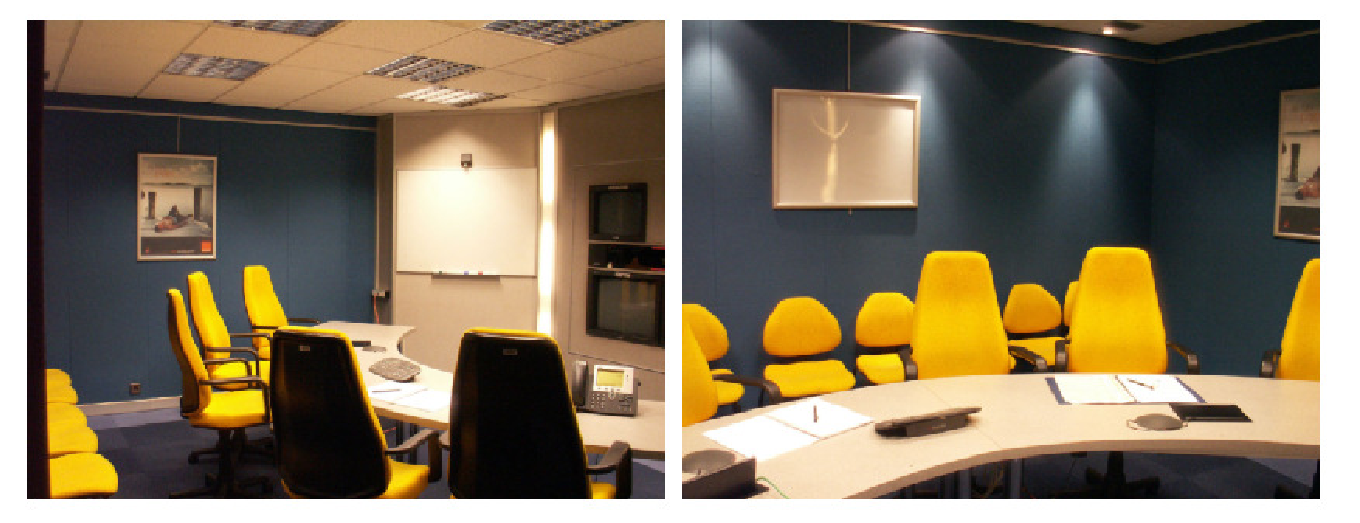
\includegraphics[scale=0.75]{video-room}
  \\
  (a) Video-conference room (Small)
  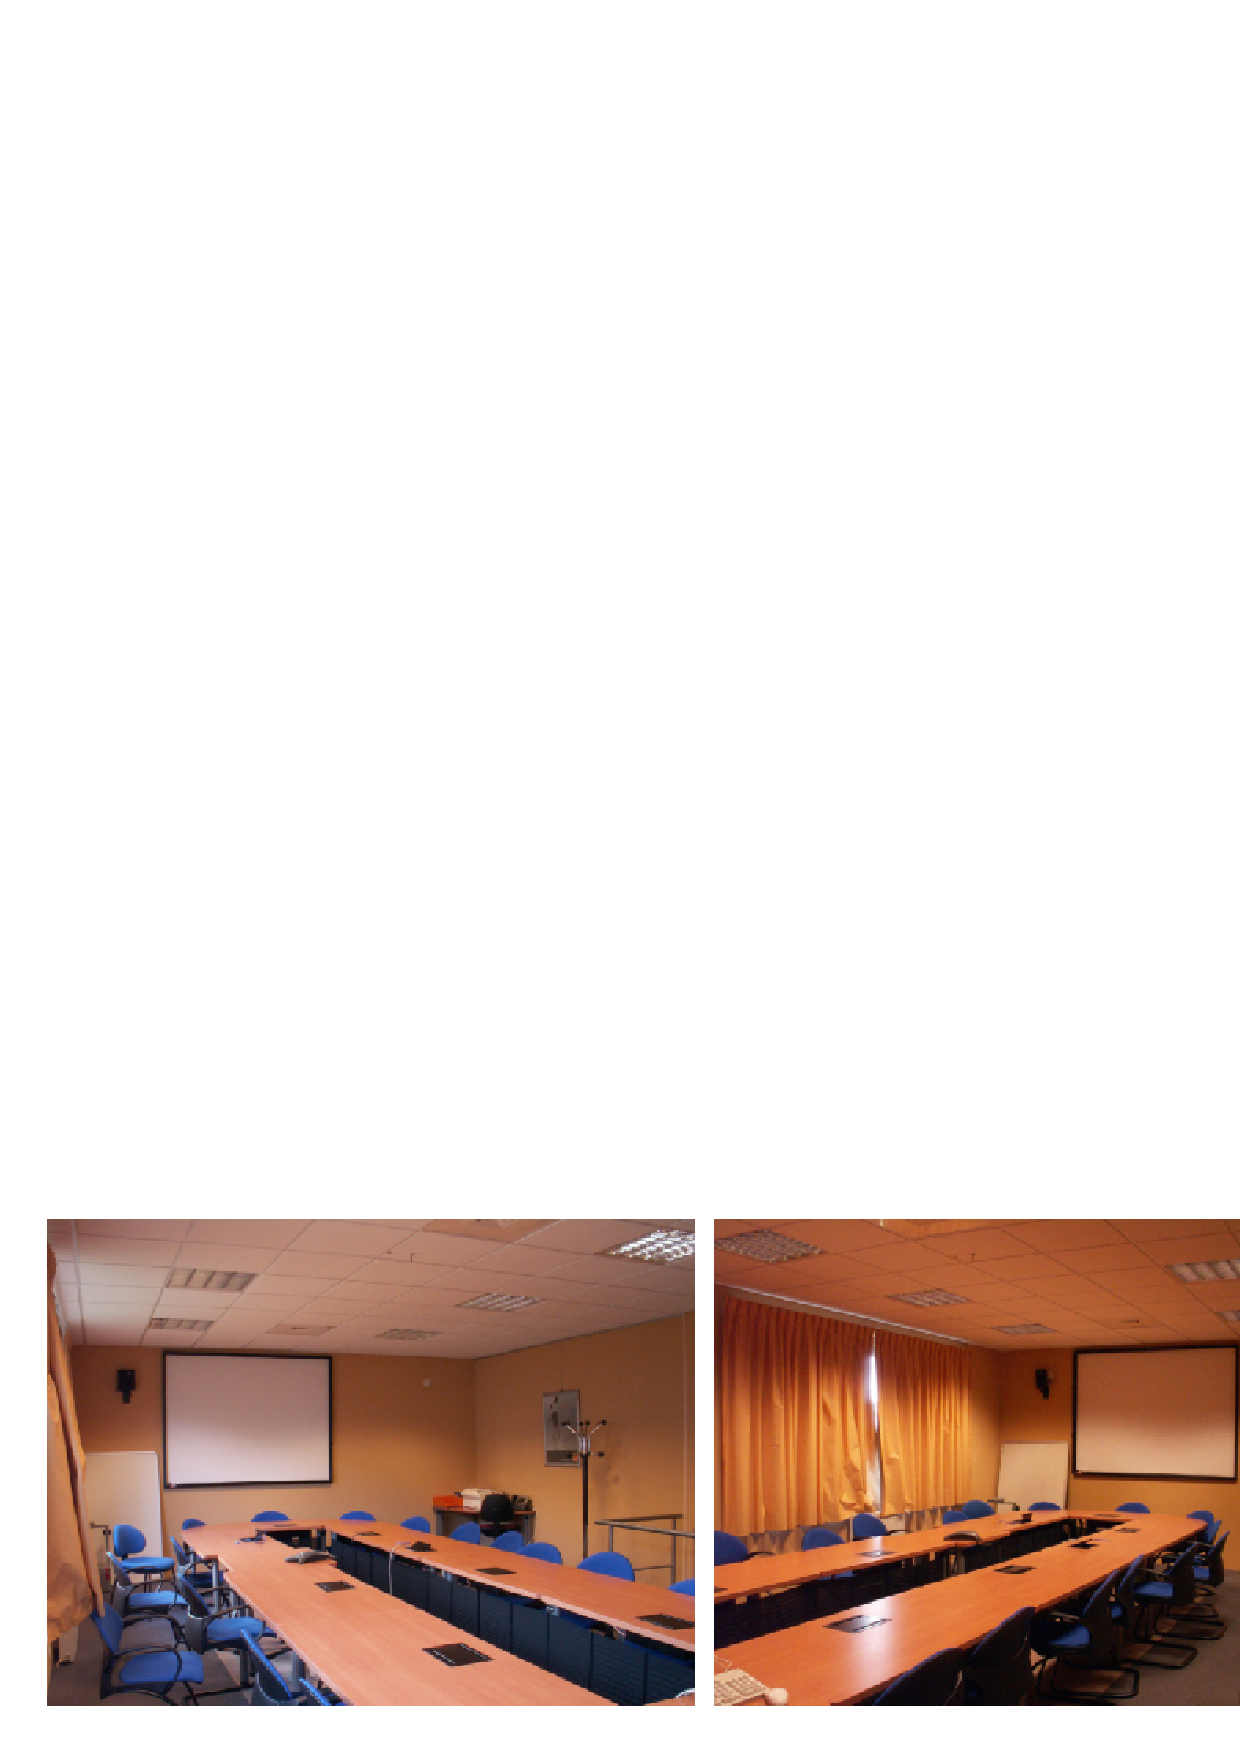
\includegraphics[scale=0.75]{meeting-room}
  \\
  (b)	Large meeting room
  \end{center}
  \caption{Pictures of the rooms where mono impulse responses sampled at 32 kHz have been measured.\label{STL05-rooms}}
\end{figure}
%------------------ End of figure ----------------------------------
\flushfloats

The geometry characteristics are given in
Table~\ref{tbl:rev-geom-room}. These rooms were acoustically treated
in order to limit the reverberation (filled carpet, acoustically
absorbent wall and ceiling). Note that the reverberation reduces the
intelligibility of recorded speech and degrades the performance of
acoustic echo canceler in case of hands-free communications.

\begin{table}
\Caption{14cm}{\SF Characteristics of the rooms where mono impulse responses sampled at 32 kHz have been measured. \label{tbl:rev-geom-room}}
\begin{center}
\begin{tabular}{|l|c|c|c|c|}
\hline & Length (m) & Width (m) &  Height (m) & Volume (m$^3$)\\
\hline Video-conference room & 4.80 & 4.45 & 2.50 & 53.40\\
\hline Meeting room & 8.55 & 5.30 & 2.70 & 122.35 \\
\hline
\end{tabular}
\end{center}
\end{table}

To give more information concerning the acoustical behaviour, the
octave-band reverberation time was computed for frequencies below 8
kHz. The values represented in Table~\ref{tbl:rev-revTime-room} were
estimated by the backward integration method applied in each
octave-band of the measured impulse response.

\begin{table}
\Caption{14cm}{\SF Octave-band reverberation time of the rooms where mono impulse responses sampled at 32 kHz have been measured.
\label{tbl:rev-revTime-room}}
\begin{center}
\begin{tabular}{|l|c|c|c|c|c|c|}
\hline
 & \multicolumn{6}{c|}{Reverberation time (ms)} \\
\hline Octave band & 125 Hz & 250 Hz & 500 Hz & 1 kHz & 2 kHz & 4
kHz \\
\hline Video-conference room & 600 & 450 & 360 & 295 & 280 &
250\\
\hline Meeting room & 671 & 600 & 518 & 490 & 466 & 440\\
\hline
\end{tabular}
\end{center}
\end{table}

%-.-.-.-.-.-.-.-.-.-.-.-.-.-.-.-.-.-.-.-.-.-.-.-.-.-.-.-.-.-.-.-.-.-.-.
\subsection{Stereo impulse response}

In STL 2009, stereo impulse responses were added. These stereo impulse
responses were measured in typical meeting rooms with various
microphones. The meeting rooms and microphone were selected according
to two scenario configurations using two rooms (one per
scenario). Pictures of the two rooms are shown in Figures
\ref{STL09-LargeMeetingRoom} and \ref{STL09-VideoConferencingRoom}.
Three types of microphone configurations were considered: MS
microphone (Sony ECM-MS907), Binaural (two omnidirectional DPA 4060
inserted into the ears of a dummy head), AB microphone (two
omnidirectional DPA 4060 microphones spaced 1 m apart).  Moreover, the
two scenarios were simulated in an anechoic room, i.e. the stereo
impulse responses were also measured in this anechoic room for all the
positions and all the microphones except for the binaural
microphone. The geometry characteristics of the large (for scenario 1)
and small (for scenario 2) rooms are given in the
Table~\ref{tbl:geom-charac-room}. These rooms were acoustically
treated in order to limit the reverberation (filled carpet,
acoustically absorbent wall and ceiling). The acoustic absorption was
higher for room of scenario 2 because the room was especially designed
for video conferencing.
\begin{table}
\Caption{14cm}{\SF Characteristics of the rooms where stereo impulse responses have been measured. \label{tbl:geom-charac-room}}
\begin{center}
\begin{tabular}{|l|c|c|c|c|}
\hline & Length (m) & Width (m) &  Height (m) & Volume (m3)\\
\hline Meeting room (Large) & 11.15	& 4.35 & 2.90 & 140.65\\
\hline Video-conference room (Small) & 5.25	& 4.75	& 2.60	& 64.83 \\
\hline
\end{tabular}
\end{center}
\end{table}

\subsubsection{Scenario 1}
The first scenario corresponds to a large conference room (see Figure \ref{STL09-LargeMeetingRoom}) with 12 
participants (12 possible positions). Figure \ref{STL09-Scenario1} shows the microphone 
configuration - AB microphone (two omnidirectional DPA 4060 microphones spaced 1.5 m apart).

%------------------------------------------------------------------------
\begin{figure}[htbp]
  \begin{center}
  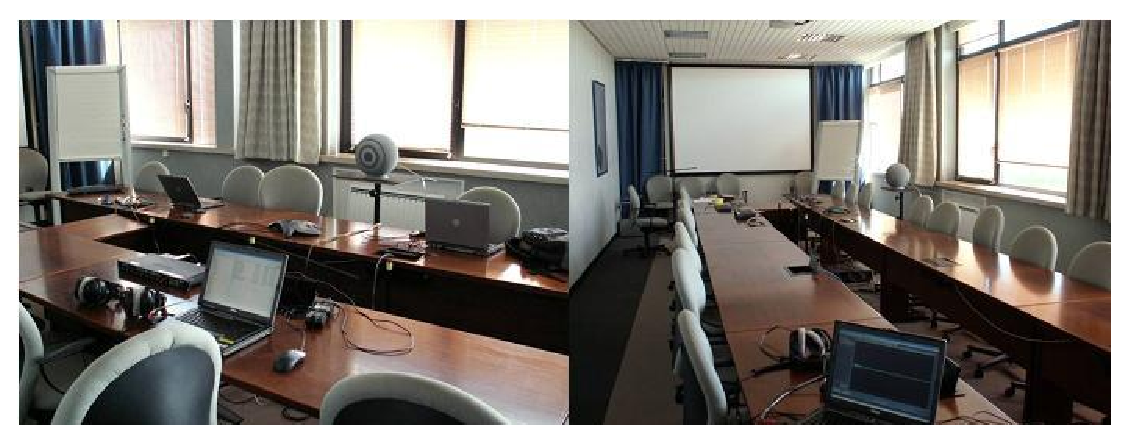
\includegraphics[scale=0.75]{LargeMeetingRoom}
  \end{center}
  \caption{Large meeting room where stereo impulse responses sampled have been measured.\label{STL09-LargeMeetingRoom}}
\end{figure}

\begin{figure}[htbp]
  \begin{center}
  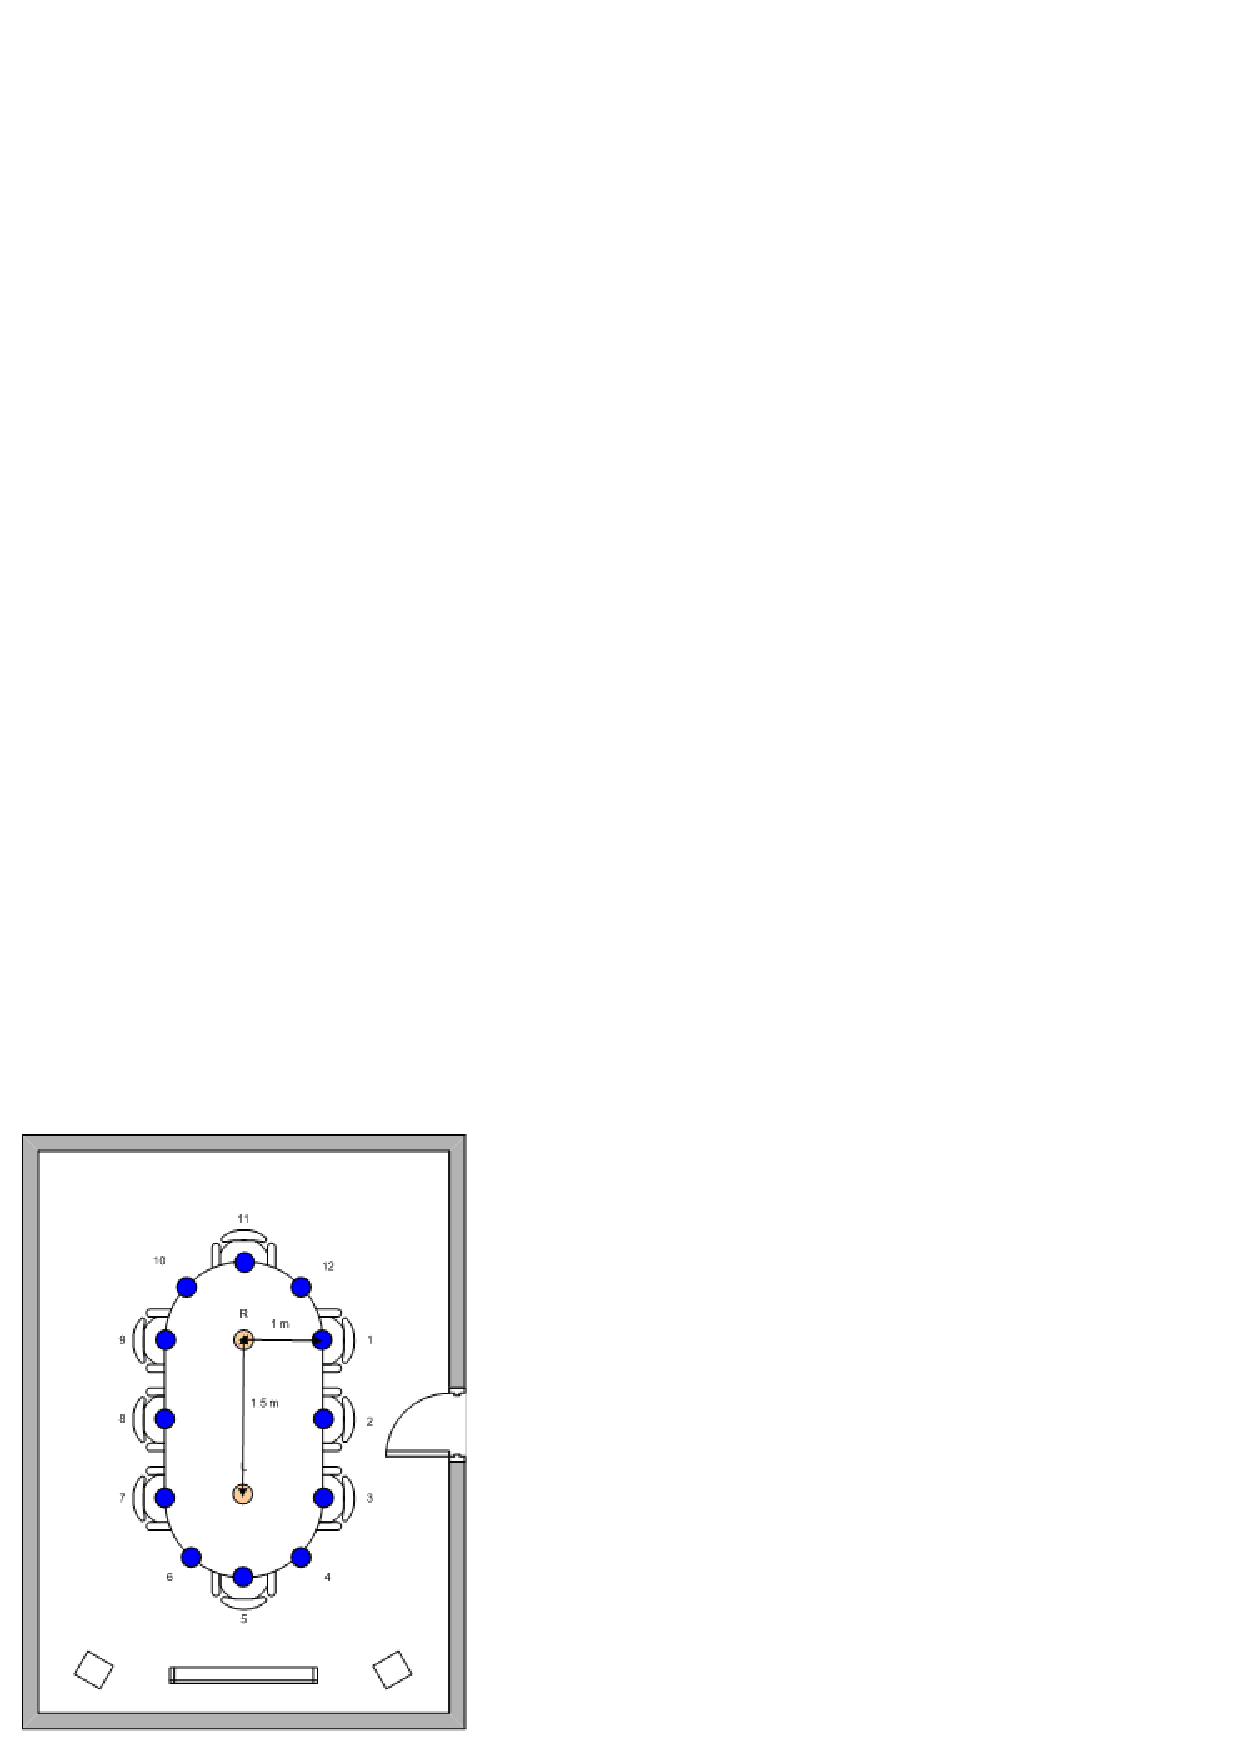
\includegraphics[scale=0.75]{Scenario1}
  \end{center}
	\caption{Scenario 1 (Large conference room, AB microphone), 
  talker positions 1 through 12.\label{STL09-Scenario1}}
\end{figure}
%------------------ End of figure ----------------------------------

\subsubsection{Scenario 2}
The second scenario corresponds to a smaller video-conference room 
 (see Figure \ref{STL09-VideoConferencingRoom}) 
with 7 seats (these seats can be positioned in 7 possible 
positions in a +/-45 degree area). Figure \ref{STL09-Scenario2} shows the microphone configurations:  MS microphone (Sony ECM-MS907), Binaural (two omnidirectional DPA 4060 inserted into the ears of a dummy head), 
AB microphone (two omnidirectional DPA 4060 microphones spaced 1 m apart).

%------------------------------------------------------------------------
\begin{figure}[htbp]
  \begin{center}
  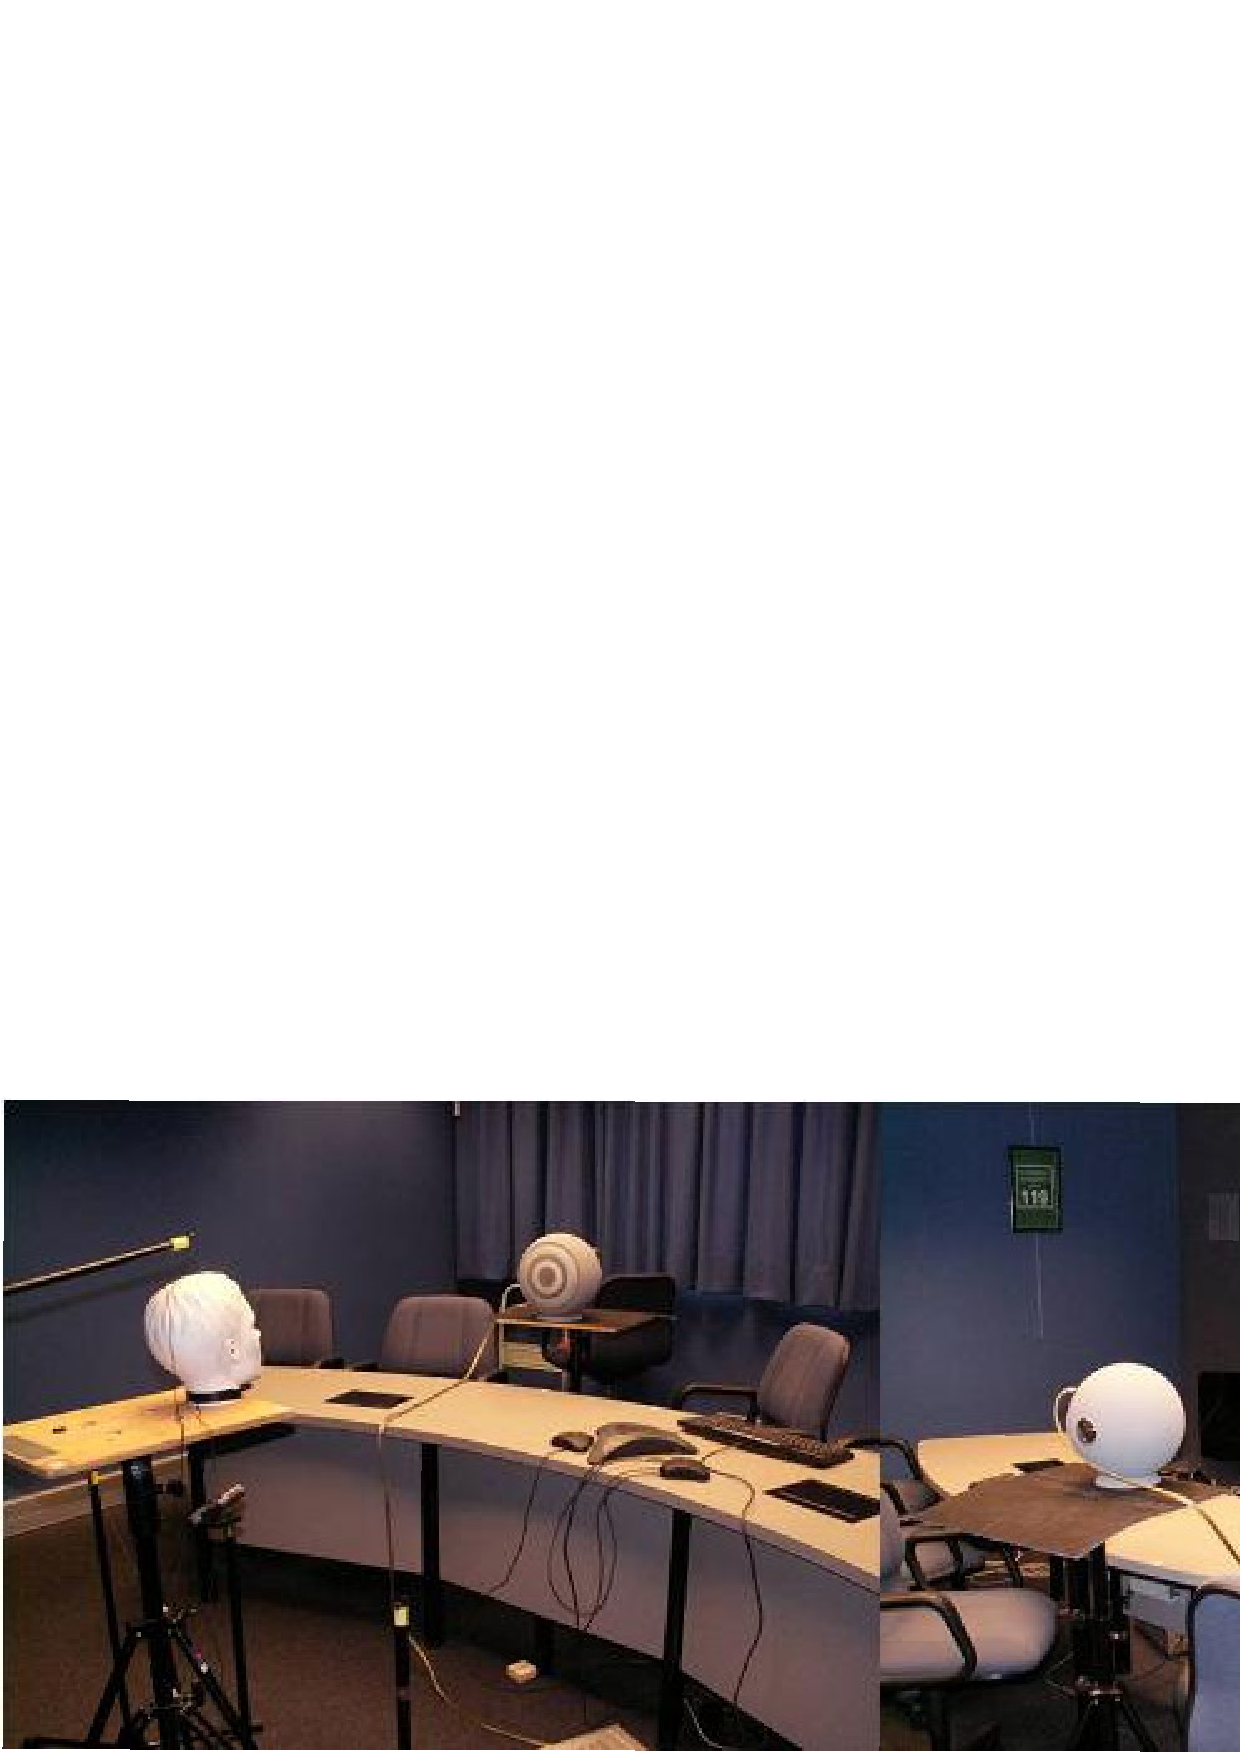
\includegraphics[scale=0.42]{VideoConferencingRoom}
  \end{center}
  \caption{Video-conference room (Small) where stereo impulse responses have been measured.\label{STL09-VideoConferencingRoom}}
\end{figure}
\begin{figure}[htbp]
  \begin{center}
  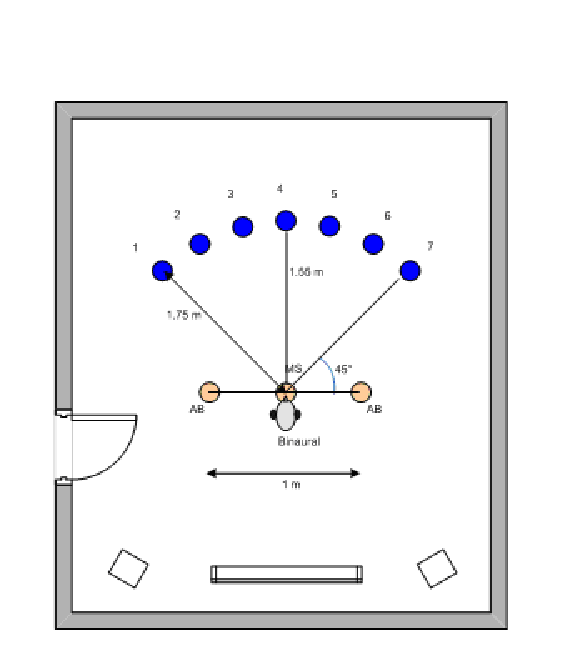
\includegraphics[scale=0.75]{Scenario2}
  \end{center}
	\caption{Scenario 2 (small video-conference room, AB, MS and 
	Binaural microphones), talker positions 1 through 7, (left though 
	right).\label{STL09-Scenario2}}
\end{figure}
%------------------ End of figure ----------------------------------
\subsubsection{List of measured stereo impulse responses}
A total of 59 stereo impulse responses have been measured resulting in 118 impulse responses. 
The naming of mono impulse responses is 
extended to include the left/right channel, further the connection to the 
room type and microphone is tabulated.

\newpage

The naming defined here is: {\tt [Room][Reverb][Mic]P[Position].[channel].IR32}, \\
where:
\begin{list}{}
\item {\tt Room} is S=Small or L=Large,
\item {\tt Reverb} is  E=Echoic or A=Anechoic,
\item {\tt Mic} is AB or MS or BI=binaural, 
\item {\tt Position} is a two digit position number, 
\item {\tt Channel} is L=Left or R=Right.
\end{list}
The detailed naming of stereo impulse responses is given in Table~\ref{tbl:nameImpulseResponse}.

\subsubsection{Office noise recording}
Office noises were recorded for the two stereo scenarios with all the
microphone configurations \cite{AC-0809-Q10-26}. The background noises
were the real sounds from air conditioner, video projector, laptop
noise (keyboard typing and fan).

%-.-.-.-.-.-.-.-.-.-.-.-.-.-.-.-.-.-.-.-.-.-.-.-.-.-.-.-.-.-.-.-.-.-.-.
\subsection{Impulse response file format}

Each sample of the IR is written in the IEEE Standard 754
floating-point representation, with both little-endian and big-endian
byte ordering and 32-bit long data type. For example, command lines
used to create the impulse responses in Matlab language were:
{\small\tt
\begin{verbatim}
fwrite(file\_identifier, impulse\_response\_vector, 'float',0,'ieee-le')
\end{verbatim}}
and
{\small\tt
\begin{verbatim}
fwrite(file\_identifier, impulse\_response\_vector, 'float',0,'ieee-be').
\end{verbatim}}
The mono Impulse Response (IR) are stored into file with ".IR"
filename extensions. The stereo IR measures are stored into files with
".IR32" filename extensions and the sampling rate is 32~kHz. When
applying these IRs, attention must be paid to have consistency between
the sampling frequency of input data and the sampling frequency of an
IR.

\begin{table}[h]
\Caption{14cm}{\SF Detailed naming of stereo impulse responses. \label{tbl:nameImpulseResponse}}
\begin{center}
\begin{tabular}{|p{7cm}|p{4.2cm}|p{3.5cm}|}
\hline
{\bf Scenario} & {\bf Main Characteristics} & {\bf Naming of impulse response pairs(with example positions):}\\
\hline
Scenario 1, Large conf. room, 12 positions, AB microphone, 
no reverb, anechoic. & Large, Anechoic, AB	& LAABP12.L.IR32 LAABP12.R.IR32\\
\hline
Scenario 1, Large conf. room, 12 positions, AB microphone, 
including reverberation.	& Large, Echoic, AB &	LEABP01.L.IR32 LEABP01.R.IR32\\
\hline
Scenario 2, small conf room, 7 positions, AB microphone, 
no reverb, anechoic. & Small, Anechoic, AB	& SAABP01.L.IR32 SAABP01.R.IR32\\
\hline
Scenario 2, small conf room, 7 positions, MS microphone, 
no reverb, anechoic.	& Small, Anechoic, MS	& SAMSP05.L.IR32 SAMSP05.R.IR32\\
\hline
Scenario 2, small conf room, 7 positions, AB microphone, 
including reverberation.	& Small, Echoic, AB	& SEABP02.L.IR32 SEABP02.R.IR32\\
\hline
Scenario 2, small conf room, 7 positions, Binaural microphone, 
including reverberation. & Small, Echoic, Binaural & SEBIP04.L.IR32 SEBIP04.R.IR32\\
\hline
Scenario 2, small conf room, 7 positions, MS microphone, 
including reverberation.	& Small, Echoic, MS	& SEMSP07.L.IR32 SEMSP07.R.IR32\\
\hline
\end{tabular}
\end{center}
\end{table}


%----------------------------------------------------------------------
\section{Implementation}
%----------------------------------------------------------------------

%-.-.-.-.-.-.-.-.-.-.-.-.-.-.-.-.-.-.-.-.-.-.-.-.-.-.-.-.-.-.-.-.-.-.-.
\subsection{\tt shift}

{\bf Syntax: }

{\tt
\#include "reverb-lib.h"\\
void shift \ttpbox{110mm}{(short* {\em buff}, long {\em N}); }}

{\bf Prototype: }    reverb-lib.h

{\bf Description: }

This routine replaces the first N-1 samples of a buffer by its
last N-1 samples. It is useful for the block-based convolution,
where N is the length of the blocks.

{\bf Variables: }
\begin{Descr}{\DescrLen}
\item[\pbox{20mm}{\em buff}] %%\rulex{1mm}\\
        buffer (input/output);

\item[\pbox{20mm}{\em N}] %%\rulex{1mm}\\
        length of each block (input);
\end{Descr}

%-.-.-.-.-.-.-.-.-.-.-.-.-.-.-.-.-.-.-.-.-.-.-.-.-.-.-.-.-.-.-.-.-.-.-.
\subsection{\tt conv}

{\bf Syntax: }

{\tt
\#include "reverb-lib.h"\\
long conv \ttpbox{110mm}{(float* {\em IR}, short* {\em buffIn},
short* {\em buffRvb}, float {\em alignFact}, long {\em N}, long
{\em L}); }}

{\bf Prototype: }    reverb-lib.h

{\bf Description: }

This function convolves the input buffer \emph{buffIn} with an
impulse response \emph{IR} and stores the processed data into the
output buffer \emph{buffRvb}. The alignment factor (multiplicative
factor) \emph{alignFact} is used to align the energy of the input
file with another file. The return value is used to provide a warning that a 16 bit saturation occurs, a positive value indicates the position of the last overflow occurrence, if no overflow occurs -1 is returned.

{\bf Variables: }
\begin{Descr}{\DescrLen}
\item[\pbox{20mm}{\em IR}] %%\rulex{1mm}\\
        impulse response buffer ;

\item[\pbox{20mm}{\em buffIn}] %%\rulex{1mm}\\
        input buffer;

\item[\pbox{20mm}{\em buffRvb}] %%\rulex{1mm}\\
        convolved data;

\item[\pbox{20mm}{\em alignFact}] %%\rulex{1mm}\\
        alignment factor;

\item[\pbox{20mm}{\em N}] %%\rulex{1mm}\\
        length of the impulse response buffer;

\item[\pbox{20mm}{\em L}] %%\rulex{1mm}\\
        length of the input buffer to process;
\end{Descr}

       {\bf Return value: }
Returns the last position of an overflow if any, otherwise -1.

%-.-.-.-.-.-.-.-.-.-.-.-.-.-.-.-.-.-.-.-.-.-.-.-.-.-.-.-.-.-.-.-.-.-.-.
\subsection{Tests and portability}

Compiled and tested on a PC (Windows) platform with MS Visual C++
6.0, in Cygwin with gcc (version 3.4.4), in Fedora 7 with gcc (version 3.4.4).

%----------------------------------------------------------------------
\section{Example code}
%----------------------------------------------------------------------

The demonstration program uses a room impulse response and a sound
file as input to produce a reverberated sound file as output. The
input sound is convolved with the room impulse response to produce
the reverberated sound. The program can be found in reverb.c.
